A Gaussian process (GP) is a collection of random variables, any finite number
of which are jointly Gaussian~\citep{rasmussen06}; it also defines a
distribution over functions on $\BBR^d$, $f \Sim \GP(\mu,k)$, where $\mu :
\BBR^d \to \BBR$ is a mean field and $k : \BBR^d \Times \BBR^d \to \BBR$ is a
symmetric and positive (semi)-definite covariance kernel. For any set of
locations $X = \{x_1,\ldots,x_n\} \binsubset \BBR^d$, $f_X \Sim \calN(\mu_X, \K
{XX})$ where $f_X$ and $\mu_X$ represent the vectors of function values for $f$
and $\mu$ evaluated at each of the $x_i \In X$, and $(\K{XX})_{ij} = k(x_i,
x_j)$.  We assume the observed function value vector $y \In \BBR^n$ is
contaminated by independent Gaussian noise with variance $\sigma^2$. We denote
any kernel hyper\hyp{}parameters by the vector $\theta$. To be concise, we
suppress the dependence of $k$ and associated matrices on $\theta$ in our
notation. Under a Gaussian process prior depending on the covariance
hyper\hyp{}parameters $\theta$, the log marginal likelihood is
given by
\begin{equation}\label{eq:mloglik}
  \calL(\theta|y) = -\frac{1}{2}\left[(y-\mu_X)^T\alpha + \log\abs{\Ktil{XX}} +
  n\log 2\pi\right]
\end{equation}
where $\alpha = \Ktil{XX}^{-1}(y-\mu_X)$ and $\Ktil{XX} = \K{XX} + \sigma^2 I$.
The standard direct method to evaluate (\ref{eq:mloglik}) and its derivatives
with respect to the hyperparameters uses the Cholesky factorization of $
\Ktil{XX}$, leading to $\calO(n^3)$ kernel learning that does not scale beyond a
few thousand points.

A popular approach to scalable GPs is to approximate the exact kernel with a
structured kernel that enables fast MVMs \citep{quinonero2005unifying}. Several
methods approximate the kernel via {\em inducing points} $U = \{u_j\}_{j=1}^m
\binsubset \BBR^d$; see, e.g.\citep{quinonero2005unifying,le2013fastfood,
hensman2013uai}. Common examples are the subset of regressors (SoR), which
exploits low-rank structure, and fully independent training conditional (FITC),
which introduces an additional diagonal correction \citep{snelson2006sparse}.
For most inducing point methods, the cost of kernel learning with $n$ data
points and $m$ inducing points scales as $\calO(m^2 n + m^3)$, which becomes
expensive as $m$ grows. As an alternative, Wilson proposed the structured kernel
interpolation (SKI) approximation,
\begin{equation}\label{eqn: ski}
  \K{XX} \approx W \K{UU} W^{T}\,,
\end{equation}
where $U$ is a uniform grid of inducing points and $W$ is an $n$-by-$m$ matrix
of interpolation weights; the authors of~\citep{wilson2015kernel} use local
cubic interpolation so that $W$ is sparse. If the original kernel is stationary,
each MVM with the SKI kernel may be computed in $\calO(n + m\log(m))$ time via
FFTs, leading to substantial performance over FITC and SoR. A limitation of SKI
is that the number of grid points increases exponentially with the dimension.
This exponential scaling has been addressed by structured kernel interpolation
for products (SKIP) \citep{gardner2018product}, which decomposes the kernel
matrix for a product kernel in $d$-dimensions as a Hadamard (elementwise)
product of one-dimensional kernel matrices.

We use fast MVMs to solve linear systems involving $\Ktil{}$ by the method of
conjugate gradients.  To estimate $\log \abs{\Ktil{}} = \tr(\log(\Ktil{}))$, we
apply stochastic trace estimators that require only products of $\log(\Ktil{})$
with random probe vectors. Given a probe vector $z$, several ideas have been
explored to compute $\log(\Ktil{}) z$ via MVMs with $\Ktil{}$, such as using a
polynomial approximation of $\log$ or using the connection between the Gaussian
quadrature rule and the Lanczos method \citep{han2015large,ubarufast}. It was
shown in \citep{dong2017scalable} that using Lanczos is superior to the
polynomial approximations and that only a few probe vectors are necessary even
for large kernel matrices.

Differentiation is a linear operator, and (assuming a twice-differentiable
kernel) we may define a multi-output GP for the function and (scaled) gradient
values with mean and kernel functions
\begin{equation}\label{eqn:meankernelderiv}
  \mu^{\nabla}(x) =
  \begin{bmatrix}
    \mu(x) \\ \dx_x \mu(x)
  \end{bmatrix}\,, \qquad
  k^{\nabla}(x,x') =
  \begin{bmatrix}
    k(x,x') & \left( \dx_{x'} k(x,x') \right)^T \\
    \dx_x k(x,x') & \ddx k(x,x')
  \end{bmatrix}\,,
\end{equation}
where $\dx_x k(x,x')$ and $\ddx^2 k(x,x')$ represent the column vector of 
(scaled) partial derivatives in $x$ and the matrix of (scaled) second partials
in $x$ and $x'$, respectively. Scaling derivatives by a natural length scale
gives the multi-output GP consistent units, and lets us understand approximation
error without weighted norms. As in the scalar GP case, we model measurements of
the function as contaminated by independent Gaussian noise.

Because the kernel matrix for the GP on function values alone is a submatrix
of the kernel matrix for function values and derivatives together, the
predictive variance in the presence of derivative information will be strictly
less than the predictive variance without derivatives. Hence, convergence of
regression with derivatives is always superior to convergence of regression
without, which is well-studied in,~e.g.~\cite[Chapter 7]{rasmussen06}. 
\cref{fig:branin} illustrates the value of derivative information; fitting with
derivatives is evidently much more accurate than fitting function values alone.
In higher-dimensional problems, derivative information is even more valuable,
but it comes at a cost: the kernel matrix $K^{\nabla}_{XX}$ is of size $n
(d+1)$-by-$n(d+1)$. Scalable approximate solvers are therefore vital in order
to use GPs for large datasets with derivative data, particularly in
high-dimensional spaces.

\begin{figure}[ht]
  \begin{center}
    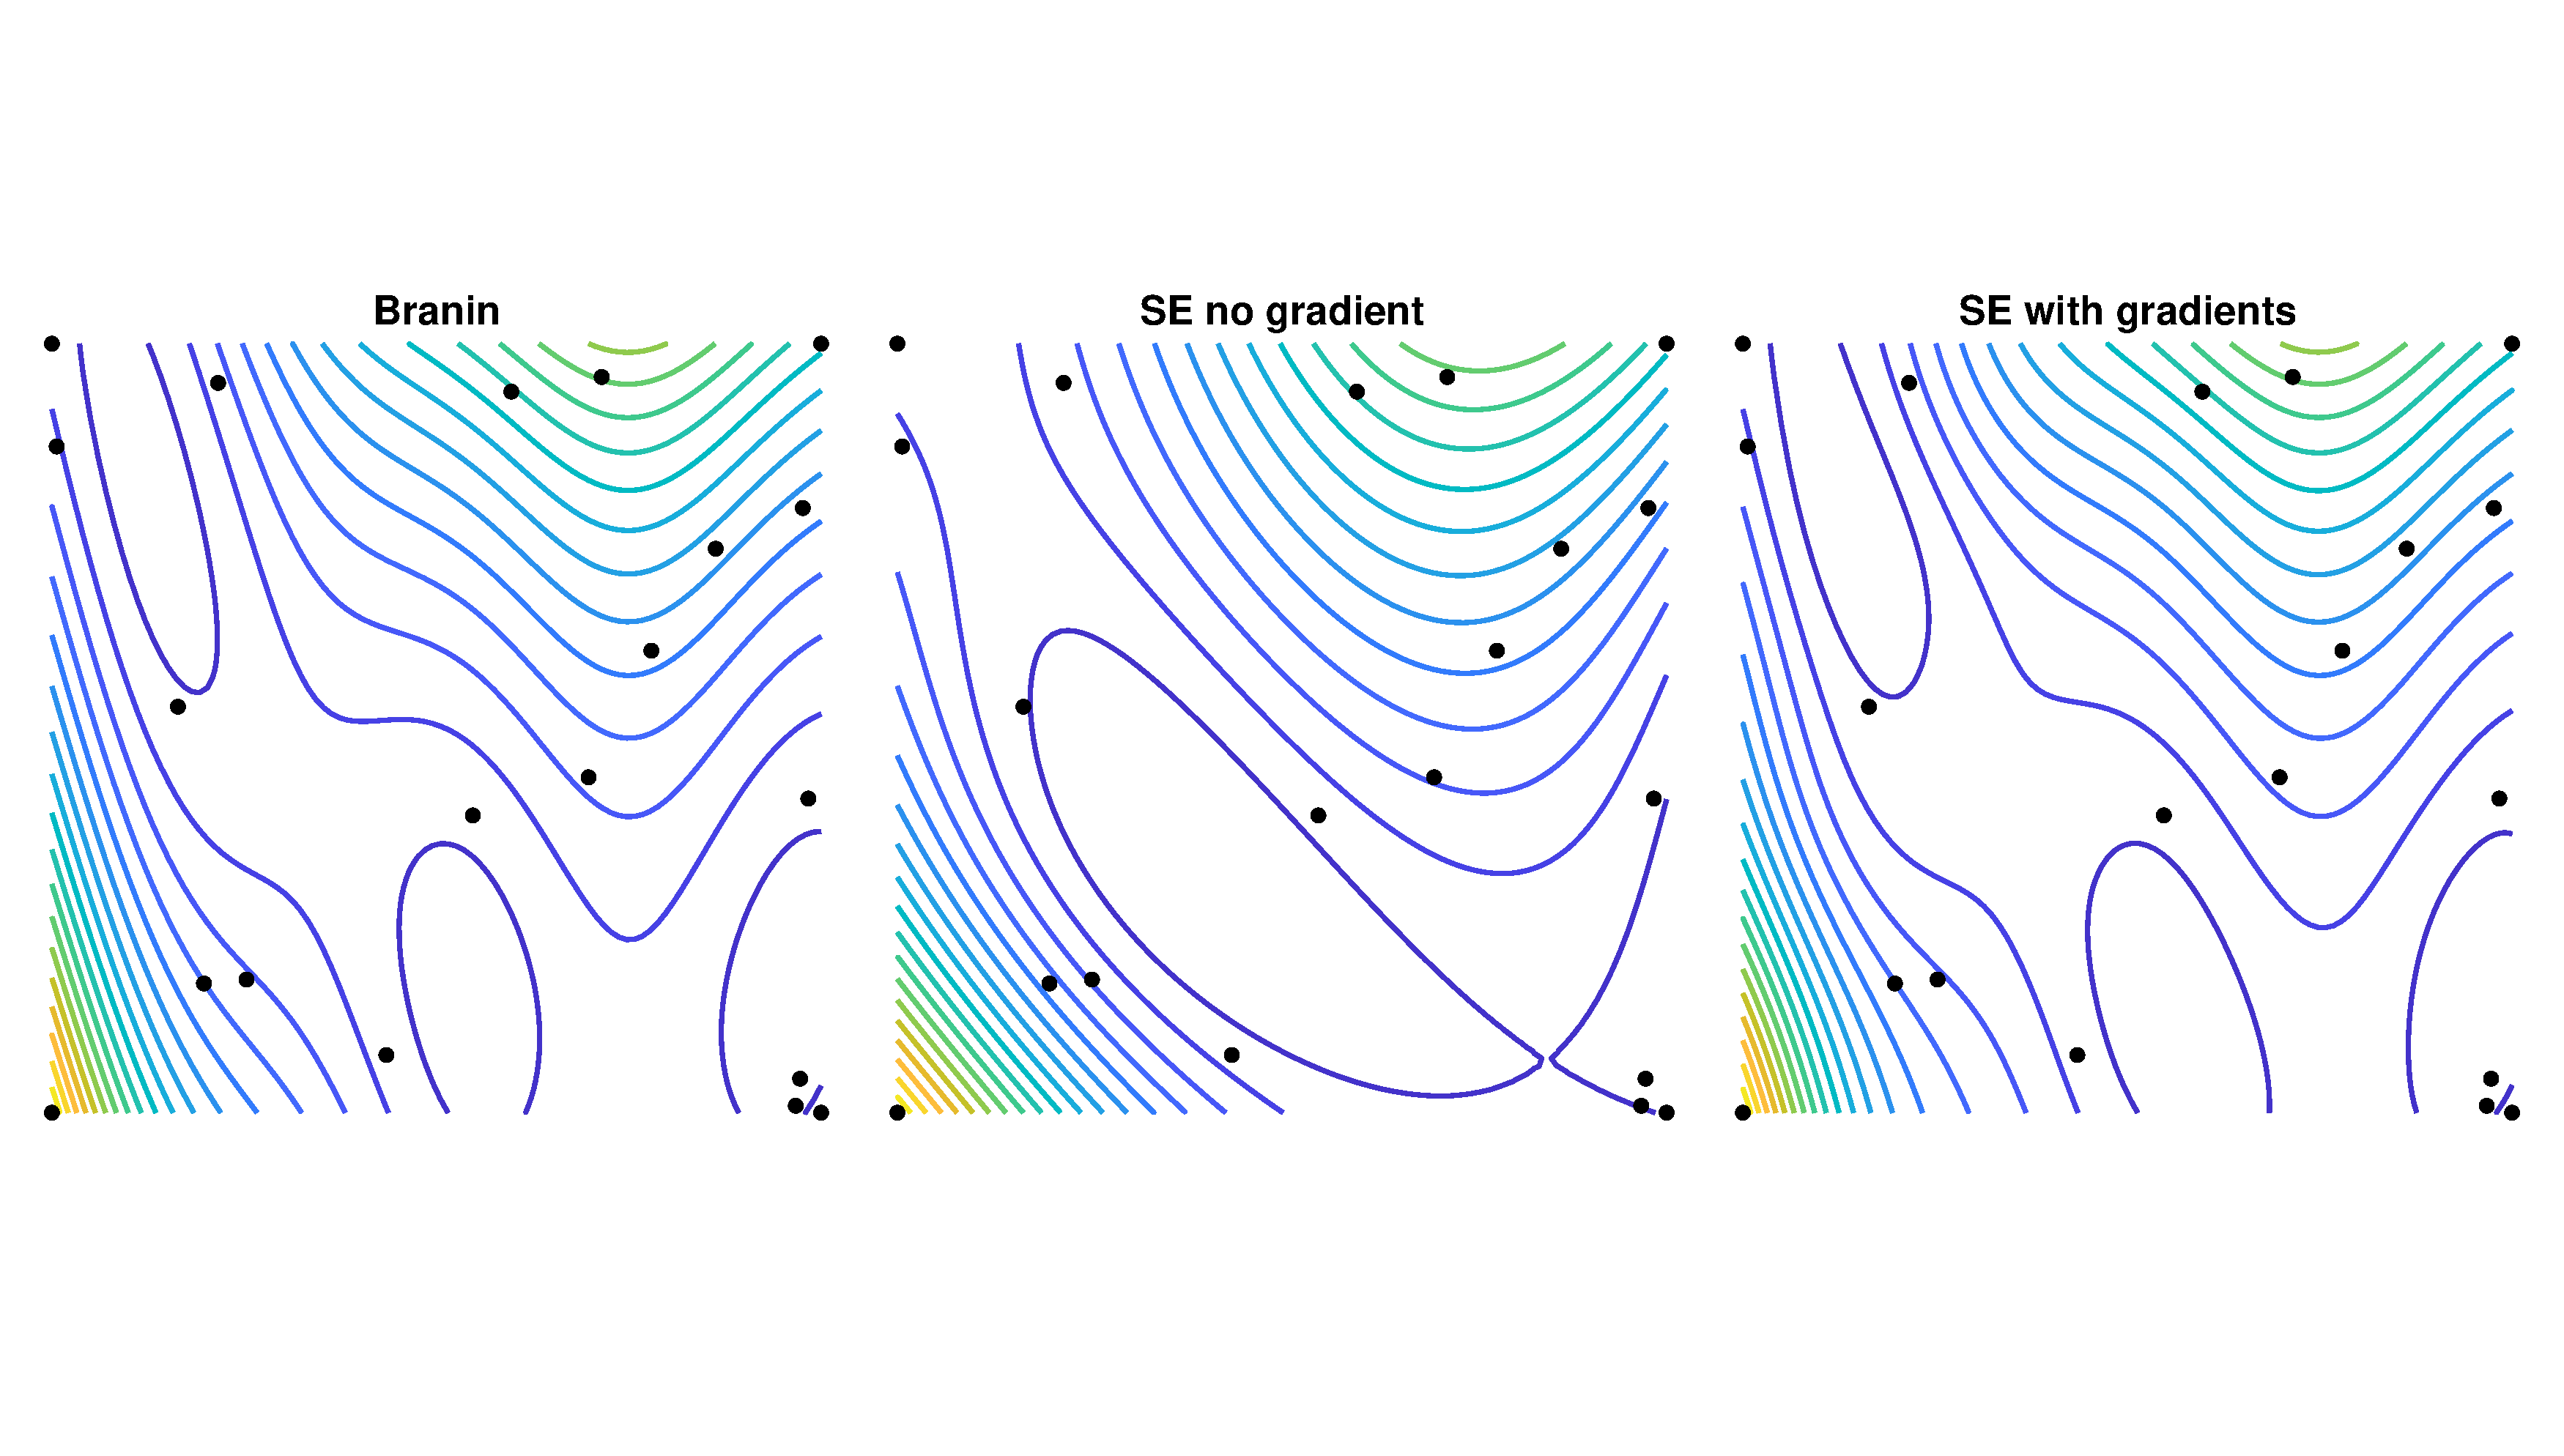
\includegraphics[width=\textwidth]{./sgpd/pics/branin}
    \caption{An example where gradient information pays off; the true function
    is on the left. Compare the regular GP without derivatives (middle) to the
    GP with derivatives (right). Unlike the former, the latter is able to
    accurately capture critical points of the function.}\label{fig:branin}
  \end{center}
\end{figure}